In this section we present a probabilistic meta-program for Bayesian
optimization, along with optimization routines implemented as concrete
applications of the meta-program.  Figure \ref{fig:slide3-definitions} shows a probabilistic meta-program for
Bayesian optimization.  We use the term ``meta-program'' because this program
defines a generic rule for combining abstract components to perform
optimization.  The components are themselves subprograms, whose implementations
may vary.  A traditional example of generic programming is the tree search
meta-program of Norvig~\cite{norvig1992paradigms}, written in LISP, which we present
alongside the optimization meta-program for comparison.

\begin{figure}[p]
  \begin{minipage}{\linewidth}
    \lstinputlisting[language=Lisp,frame=single]{sections/norvig_search.lisp}
    \lstinputlisting[language=Venture,frame=single]{sections/generic_bayesopt.scm}
  \end{minipage}
  \caption{
    Top: Norvig's LISP meta-program for tree search.
    Bottom: A probabilistic meta-program for Bayesian optimization, written in
    VentureScheme, an abstract, Scheme-like syntax that can be used for Venture.
  }
  \label{fig:slide3-definitions}
\end{figure}

Figure \ref{fig:slide3-tree-search} shows the flexibility of Norvig's
meta-program.  The procedure \texttt{tree-search} can be turned into a concrete
implementation of depth-first, breadth-first or best-first search (among others)
by simply supplying the appropriate combiner and set of initial states.
Similarly, the meta-procedure \texttt{optimize} can make use of a variety of
statistical emulators (e.g., GP-based emulators or polynomial regressions), a
variety of acquisition heuristics (e.g., randomized grid search or Gaussian
drift) and even a variety of rules for choosing an optimum based on the final
state of the program (e.g., return the best probe so far, or return the
analytically determined optimum of the emulator). 

\begin{figure}
  \centering
  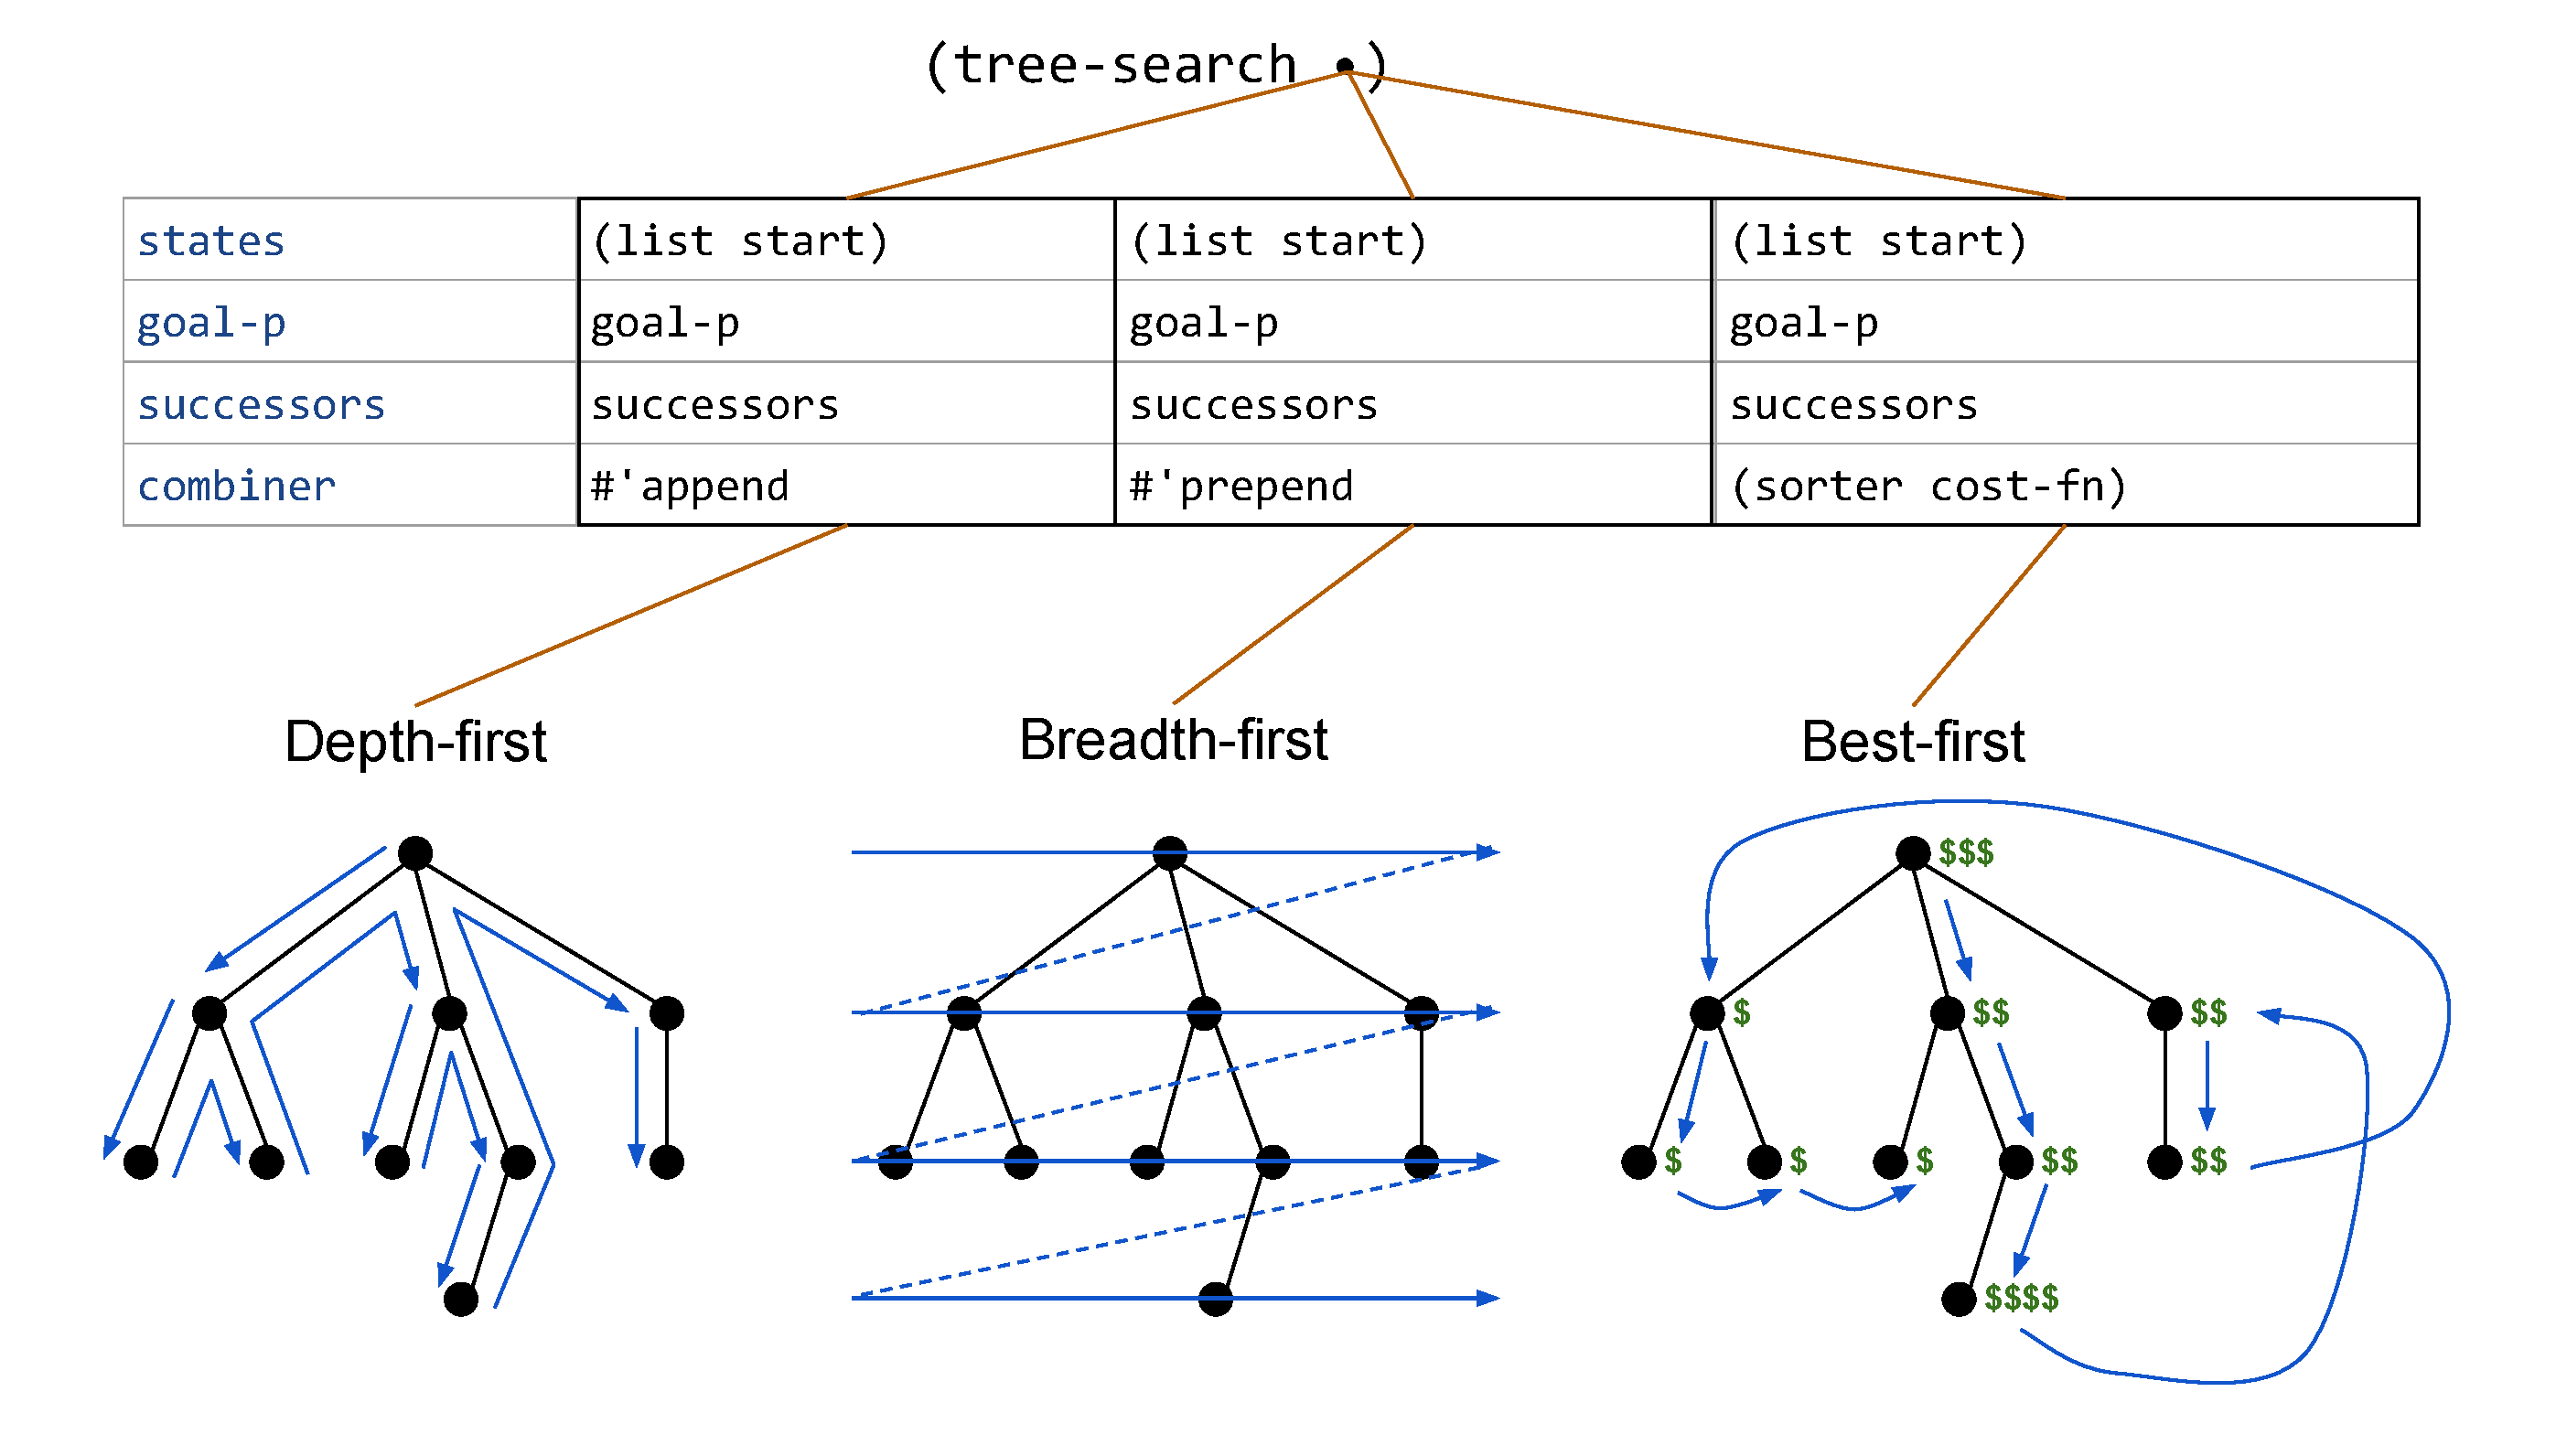
\includegraphics[width=\linewidth]{slides/slide3_treesearch.pdf}
  \caption{
    Invocations of Norvig's tree search meta-procedure with different arguments
    to perform a variety of different tree searches.
  }
  \label{fig:slide3-tree-search}
\end{figure}


The specifications for the arguments to the meta-procedure \texttt{optimize} in
Figures \ref{fig:slide3-definitions} are as
follows:
\newcommand{\itmh}[1]{\textbf{\texttt{#1}:}}
\begin{itemize}
  \item \itmh{probe}
    A procedure for querying the true function $\ftt$ (and storing its
    value in the appropriate table, if caching is desired).
  \item \itmh{do\_search}
    A procedure to search for a new probe point and, if one is found, store it
    in \texttt{search\_state\_box}.
  \item \itmh{search\_state\_box}
    A container for the next value to be probed.  In each iteration of the loop,
    if the contents of \texttt{search\_state\_box} have changed, a new probe is
    performed.
  \item \itmh{post\_probe\_inference}
    Any inference instructions which should be run after each probe, such
    as inferring hyperparameters.
  \item \itmh{extract\_answer}
    A procedure to produce an approximate optimum, based on the probes and
    inference that have been done so far.
  \item \itmh{finished?}
    A procedure to decide whether optimization should be truncated here or
    should continue.
\end{itemize}
The meta-program is quite simple: Until \texttt{finished?} decides that
optimization is finished, we choose new probe points and call
\texttt{probe} on them.  After each probe, we perform post-probe inference.
Once optimization is finished, we call \texttt{extract\_answer} to obtain
an approximate optimum.
